\documentclass[a4paper]{article}

\usepackage[T1]{fontenc}
\usepackage{titling}
\usepackage[polish]{babel}
\selectlanguage{polish}
\usepackage[utf8]{inputenc}
\usepackage{amsmath}
\usepackage{amsfonts}

\usepackage{framed}
\usepackage{fullpage}
\usepackage{graphicx}
\usepackage{diagbox}

\usepackage{textcomp}
\usepackage{float}
\usepackage{gensymb}
\usepackage{tabularx,ragged2e,booktabs,caption}
\usepackage{subfigure}
\usepackage{multicol,tabularx,capt-of}
\usepackage{multirow}
\usepackage{adjustbox}
\usepackage{algpseudocode}
\usepackage{physics}
\usepackage{listings}
\lstset
{ 
    basicstyle=\small,
    numbers=left,
    stepnumber=1,
    showstringspaces=false,
    tabsize=1,
    breaklines=true,
}

\setlength{\droptitle}{+10em}
\title{\huge JD \\
	\large Programowanie zespołowe}
\author{Jakub Brodziński \\ 229781}
\date{}

\begin{document}
\maketitle
\pagebreak
\section{Wstęp}
\section{Analiza problemu}
\section{Projekt systemu}
\subsection{Architektura projektu}
Cieżko jest mówić o naszej aplikacji jak o jednym bycie, ponieważ można ją podzielić na dwa podsystemu, gdzie w obu przypadkach archiktektura systemu jest wielowarstwowa. Jednym z podsystemów jest aplikacja webowa, która została zaprojektowana w oparciu o wzorzec \textbf{MVC} (ang. Model-View-Controller), który to narzucił wielowarstwową architektura. Oddzielając logikę biznesową od modelu (tj. danych) oraz interfejsu użytkownika aplikacji została zaprojektowana zgodnie z zasadami \textbf{GRASP} (ang. General responsibility assignment software patterns). Taka a nie inna architektura aplikacji webowej oprócz znacznego zwiększenia czytelności kodu pozwoliła na wielowarstwowe zabezpieczenia, które zostały nałożone na każdą z trzech głównych warstw naszej aplikacji. Samą część łącząca wartswe modelu oraz controller'a możemy podzielić na dwie podwarstwy: \textbf{DAO} (ang. Data Access Object) oraz \textbf{Service}.
\begin{figure}[H]
  \centering
  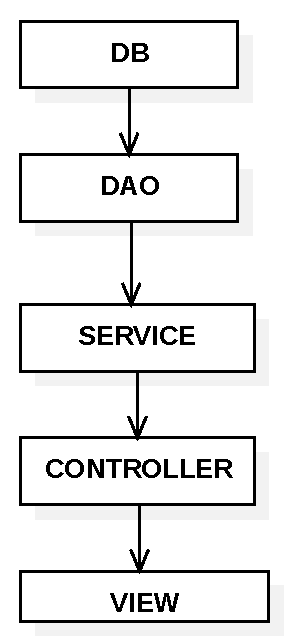
\includegraphics[scale=0.6]{diagram1.pdf}
  \caption{System podzielony na podwarstwy.}
\end{figure}
Warstwa \textbf{DAO} odpowiedzialna jest bezpośrednio na komunikacje z wartswą modelu, tj. bazą danych. Natomiast to w warstwie serwisowej, która korzysta z warstwy \textbf{DAO} została zaimplementowana cała logika biznesowa i to właśnie z warstwy serwisowej korzystamy w kontrolerach.
\linebreak
Drugim podsystemem naszego projektu jest aplikacja webowa, która również jest systemem rozproszonym komunikującym się z serwerem (który jest częścią pierwszego podsystemu) wykorzystując \textbf{REST} (ang. Representational State Transfer) oferując użytkownikowi jedynie część funkcjonalności aplikacji webowej.
\linebreak
W projekcie poza stosowaniem zasad \textbf{GRASP} zostały wykorzystane takie wzorce projektowe jak \textbf{Proxy}, \textbf{Template Method}, \textbf{Adapter}, \textbf{Factory} oraz \textbf{Decorator}, \textbf{Dependency Injection}, \textbf{Aspect Oriented Programing}, \textbf{Singleton}, które w sposób naturalny współgrały z użytymi przez nas technologiami.
\subsection{Przypadki użycia i scenriusze}
\subsection{Diagramy klas}
Diagramy przedstawione poniżej przedstawiają klasy serwisowe, w których to właśnie została zaimplementowana cała logika biznesowa naszego systemu  i to one reprezentują funkcjonalność i możliwości naszej aplikacji webowej. W celu zwiększenia czytelności diagramów z ich większości zostały usunięte trywialne metody (nie zawierające logiki biznesowej), których zadaniem było dodanie, edycja, usunięcie przekazywanego obiektu w bazie danych.
\begin{figure}[H]
  \centering
  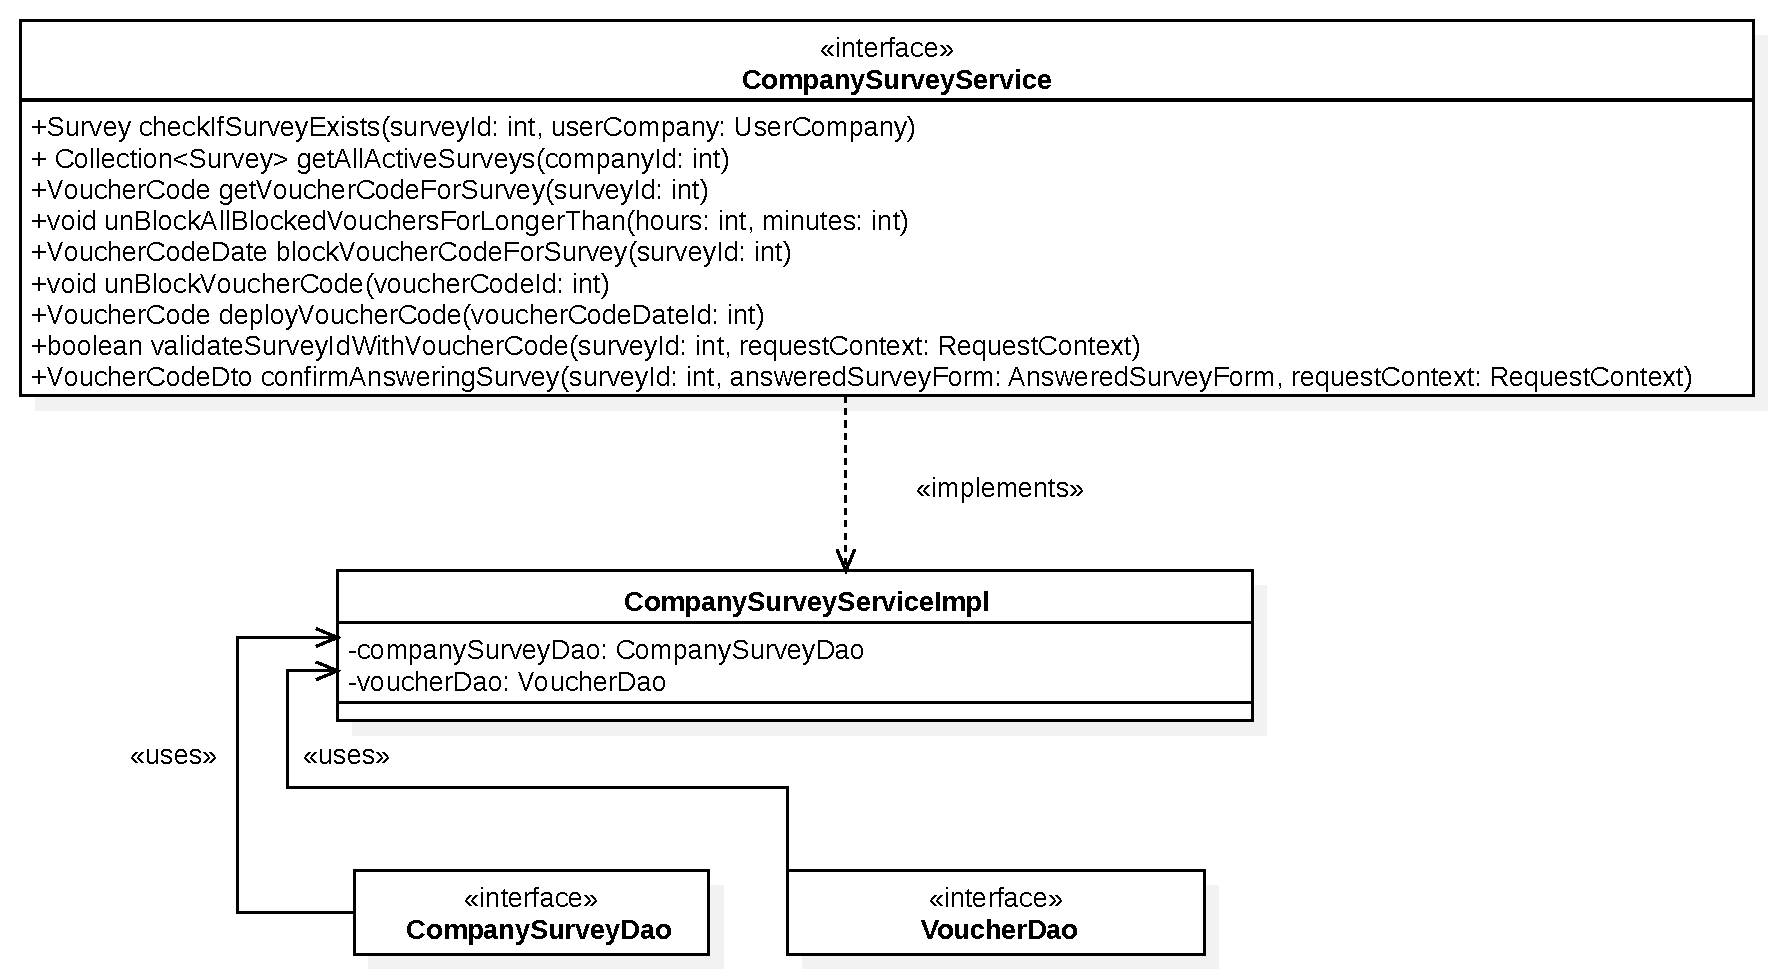
\includegraphics[scale=0.6]{company_survey_service.pdf}
  \caption{Diagram klas dla interfejsu serwisowego $CompanySurveyService$}
\end{figure}
Powyższy diagram przedstawia diagram klas dla serwisu, który przede wszystskim obsługuje funkcjonalność związana pobieraniem aktywnym, przeglądaniem oraz wypełnianiem ankiet jak również walidacją tych czynności. Ponadto odpowiedzialny jest za podjęcie decyzji czy dany kupon powininen zostać wydany czy też nie.
\begin{figure}[H]
  \centering
  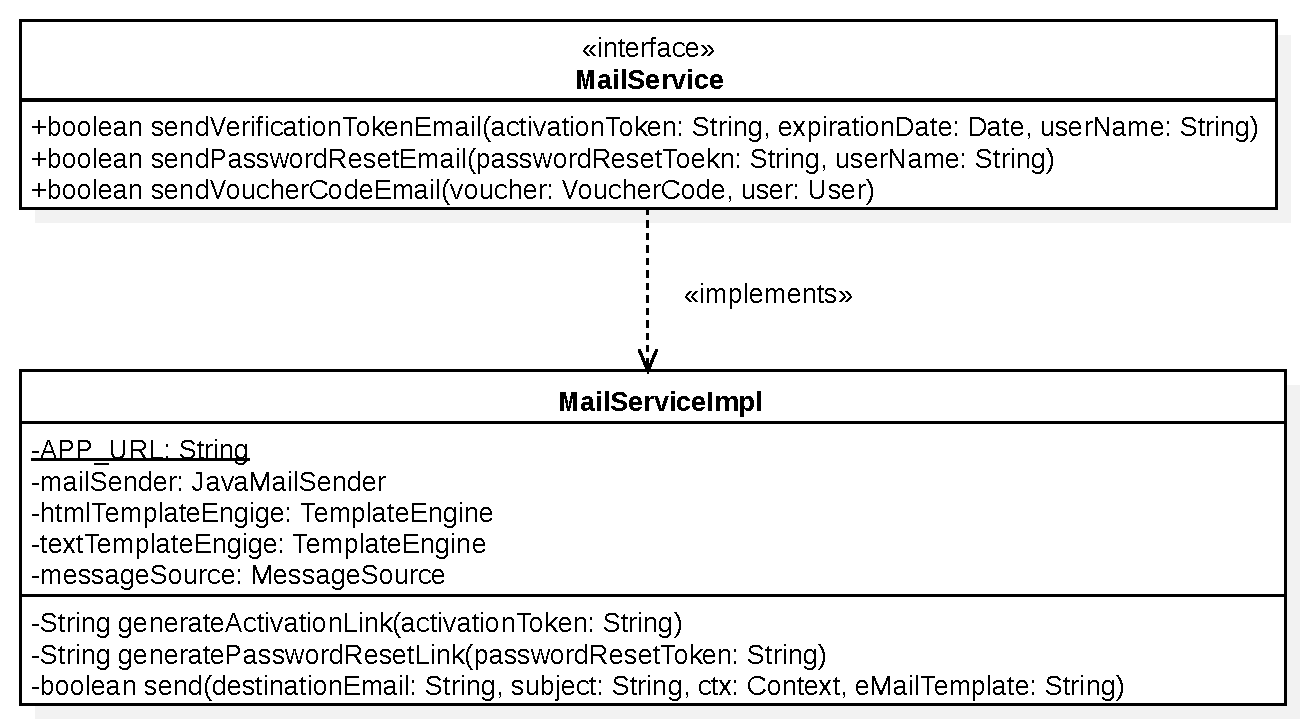
\includegraphics[scale=0.6]{mail_service.pdf}
  \caption{Diagram klas dla interfejsu serwisowego $MailService$}
\end{figure}
W \textbf{MailService} każda metoda odpowiada innemu typu  wiadomości, która zostanie wysłąna.
\begin{figure}[H]
  \centering
  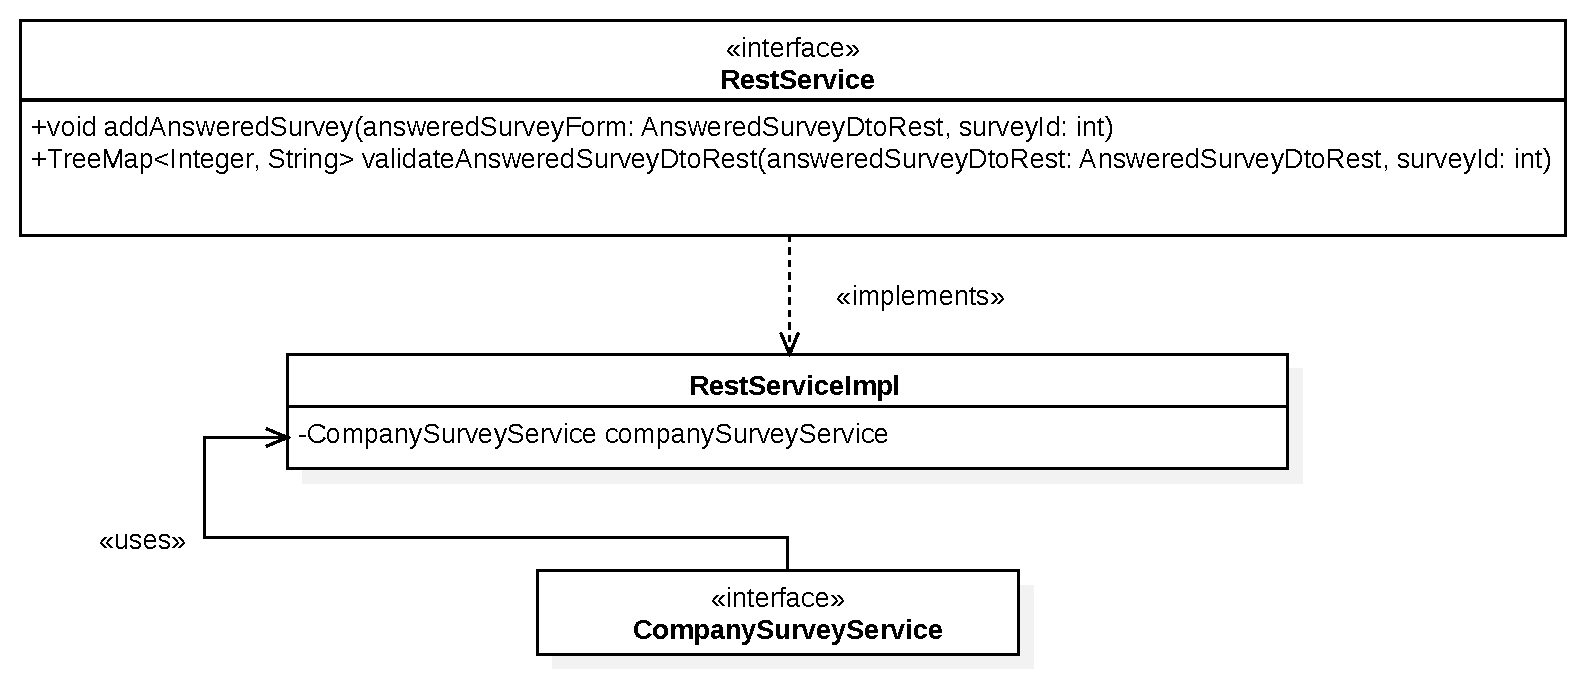
\includegraphics[scale=0.6]{rest_service.pdf}
  \caption{Diagram klas dla interfejsu serwisowego $RestService$}
\end{figure}
Powyższy diagram klas przedstawia diagram klas serwisowych obsługujących \textbf{REST Api}, które jest wykorzystywane przez aplikacje mobilna.
\begin{figure}[H]
  \centering
  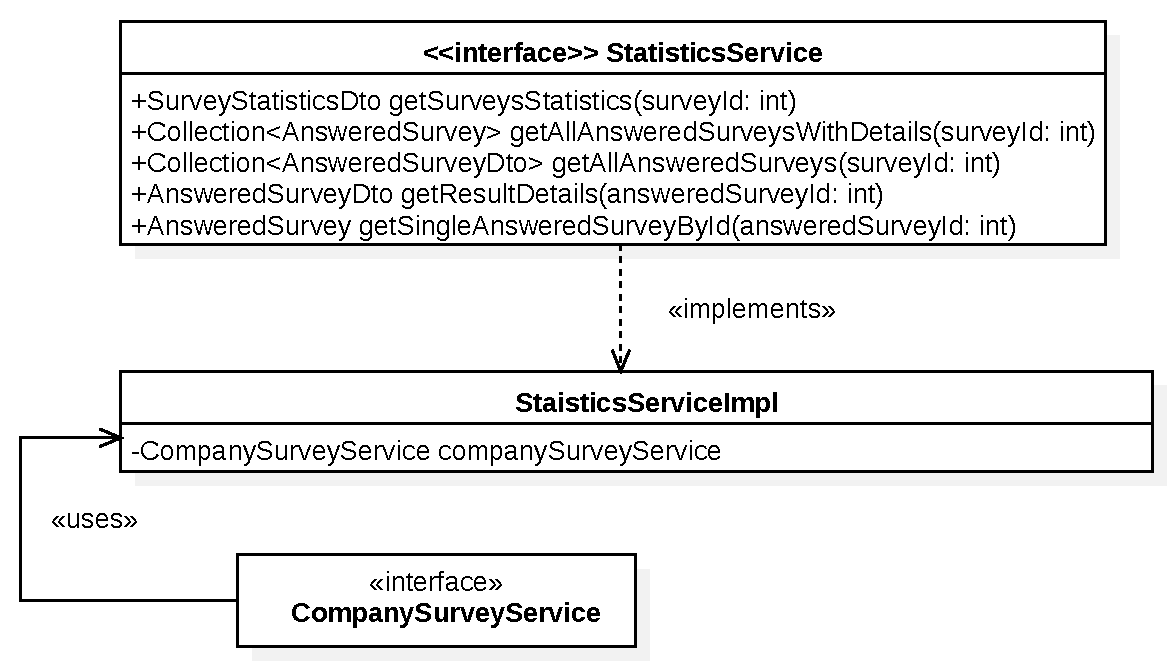
\includegraphics[scale=0.6]{statistics_service.pdf}
  \caption{Diagram klas dla interfejsu serwisowego $StatisticsService$}
\end{figure}
W powyżej przedstawionych klasach serwisowych obliczane są statystyki, które każdy użytkownik ze stworzonymi ankietami może przeglądać.
\begin{figure}[H]
  \centering
  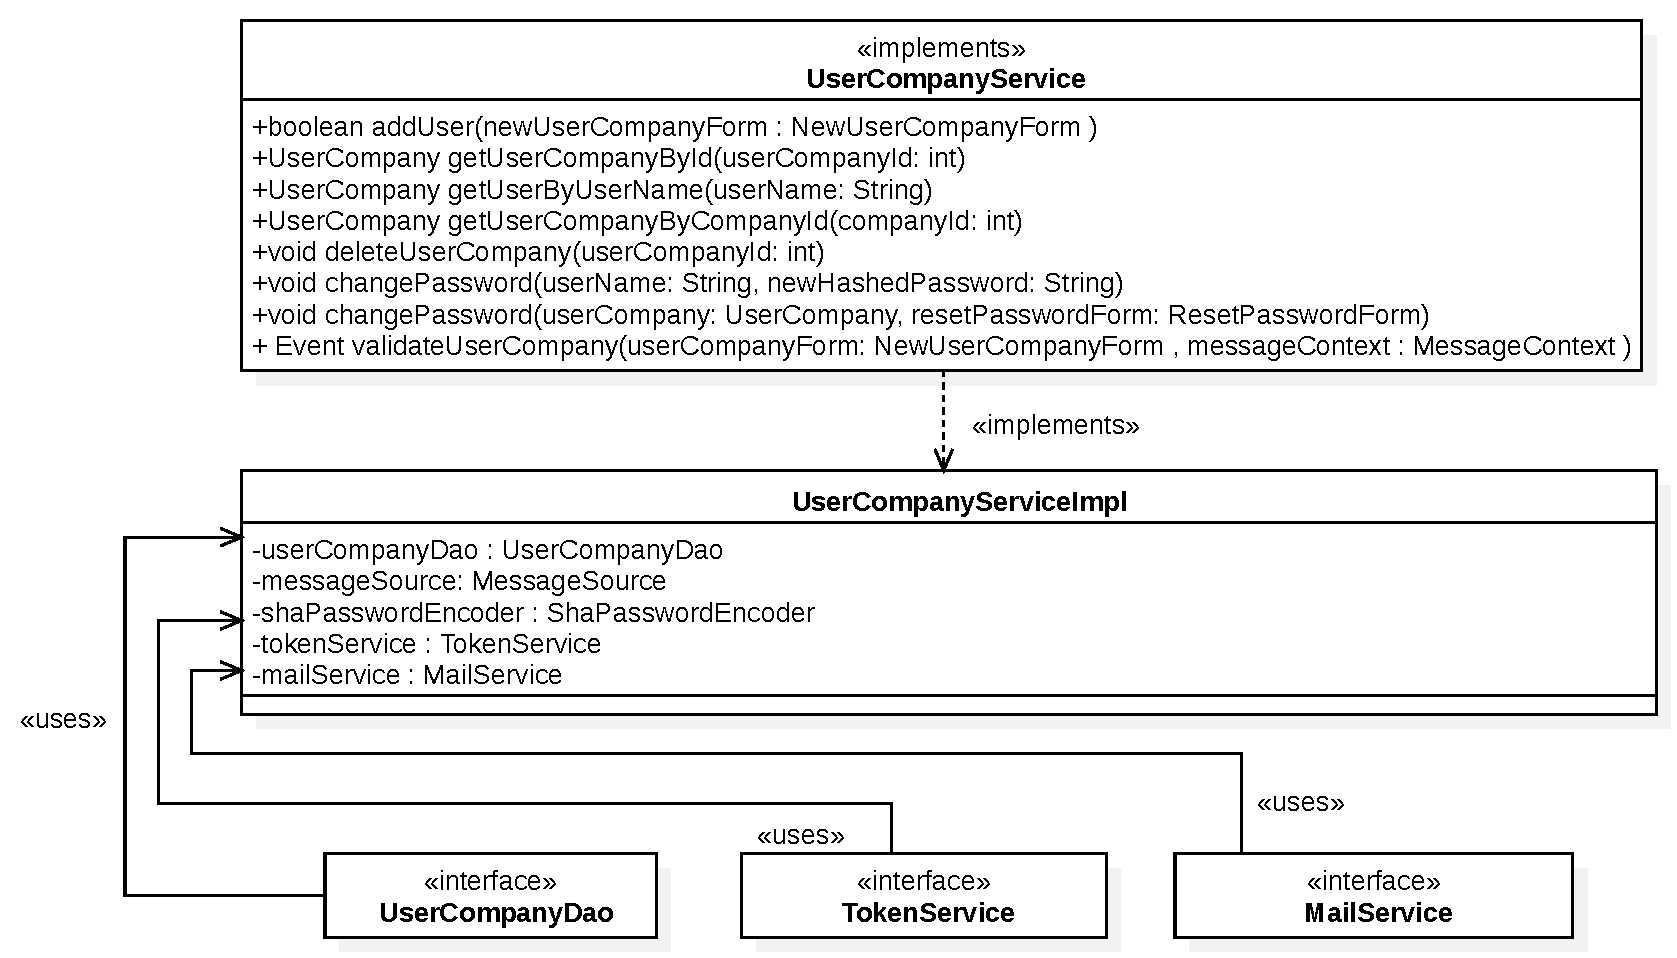
\includegraphics[scale=0.6]{user_company_service.pdf}
  \caption{Diagram klas dla interfejsu serwisowego $UserCompanyService$}
\end{figure}
Klasy serwisowe w diagramie powyżej odpowiadają za część funckjonalności związanej z kontem firmy, tj. edycja danych, rejestracja, logowanie, zmiana hasła itd.
\subsection{Diagramy aktywności}
\subsection{Diagramy sekwencji}
\subsection{Diagramy stanów}
\pagebreak
\subsection{Projekt bazy danych}
\begin{figure}[H]
  \centering
  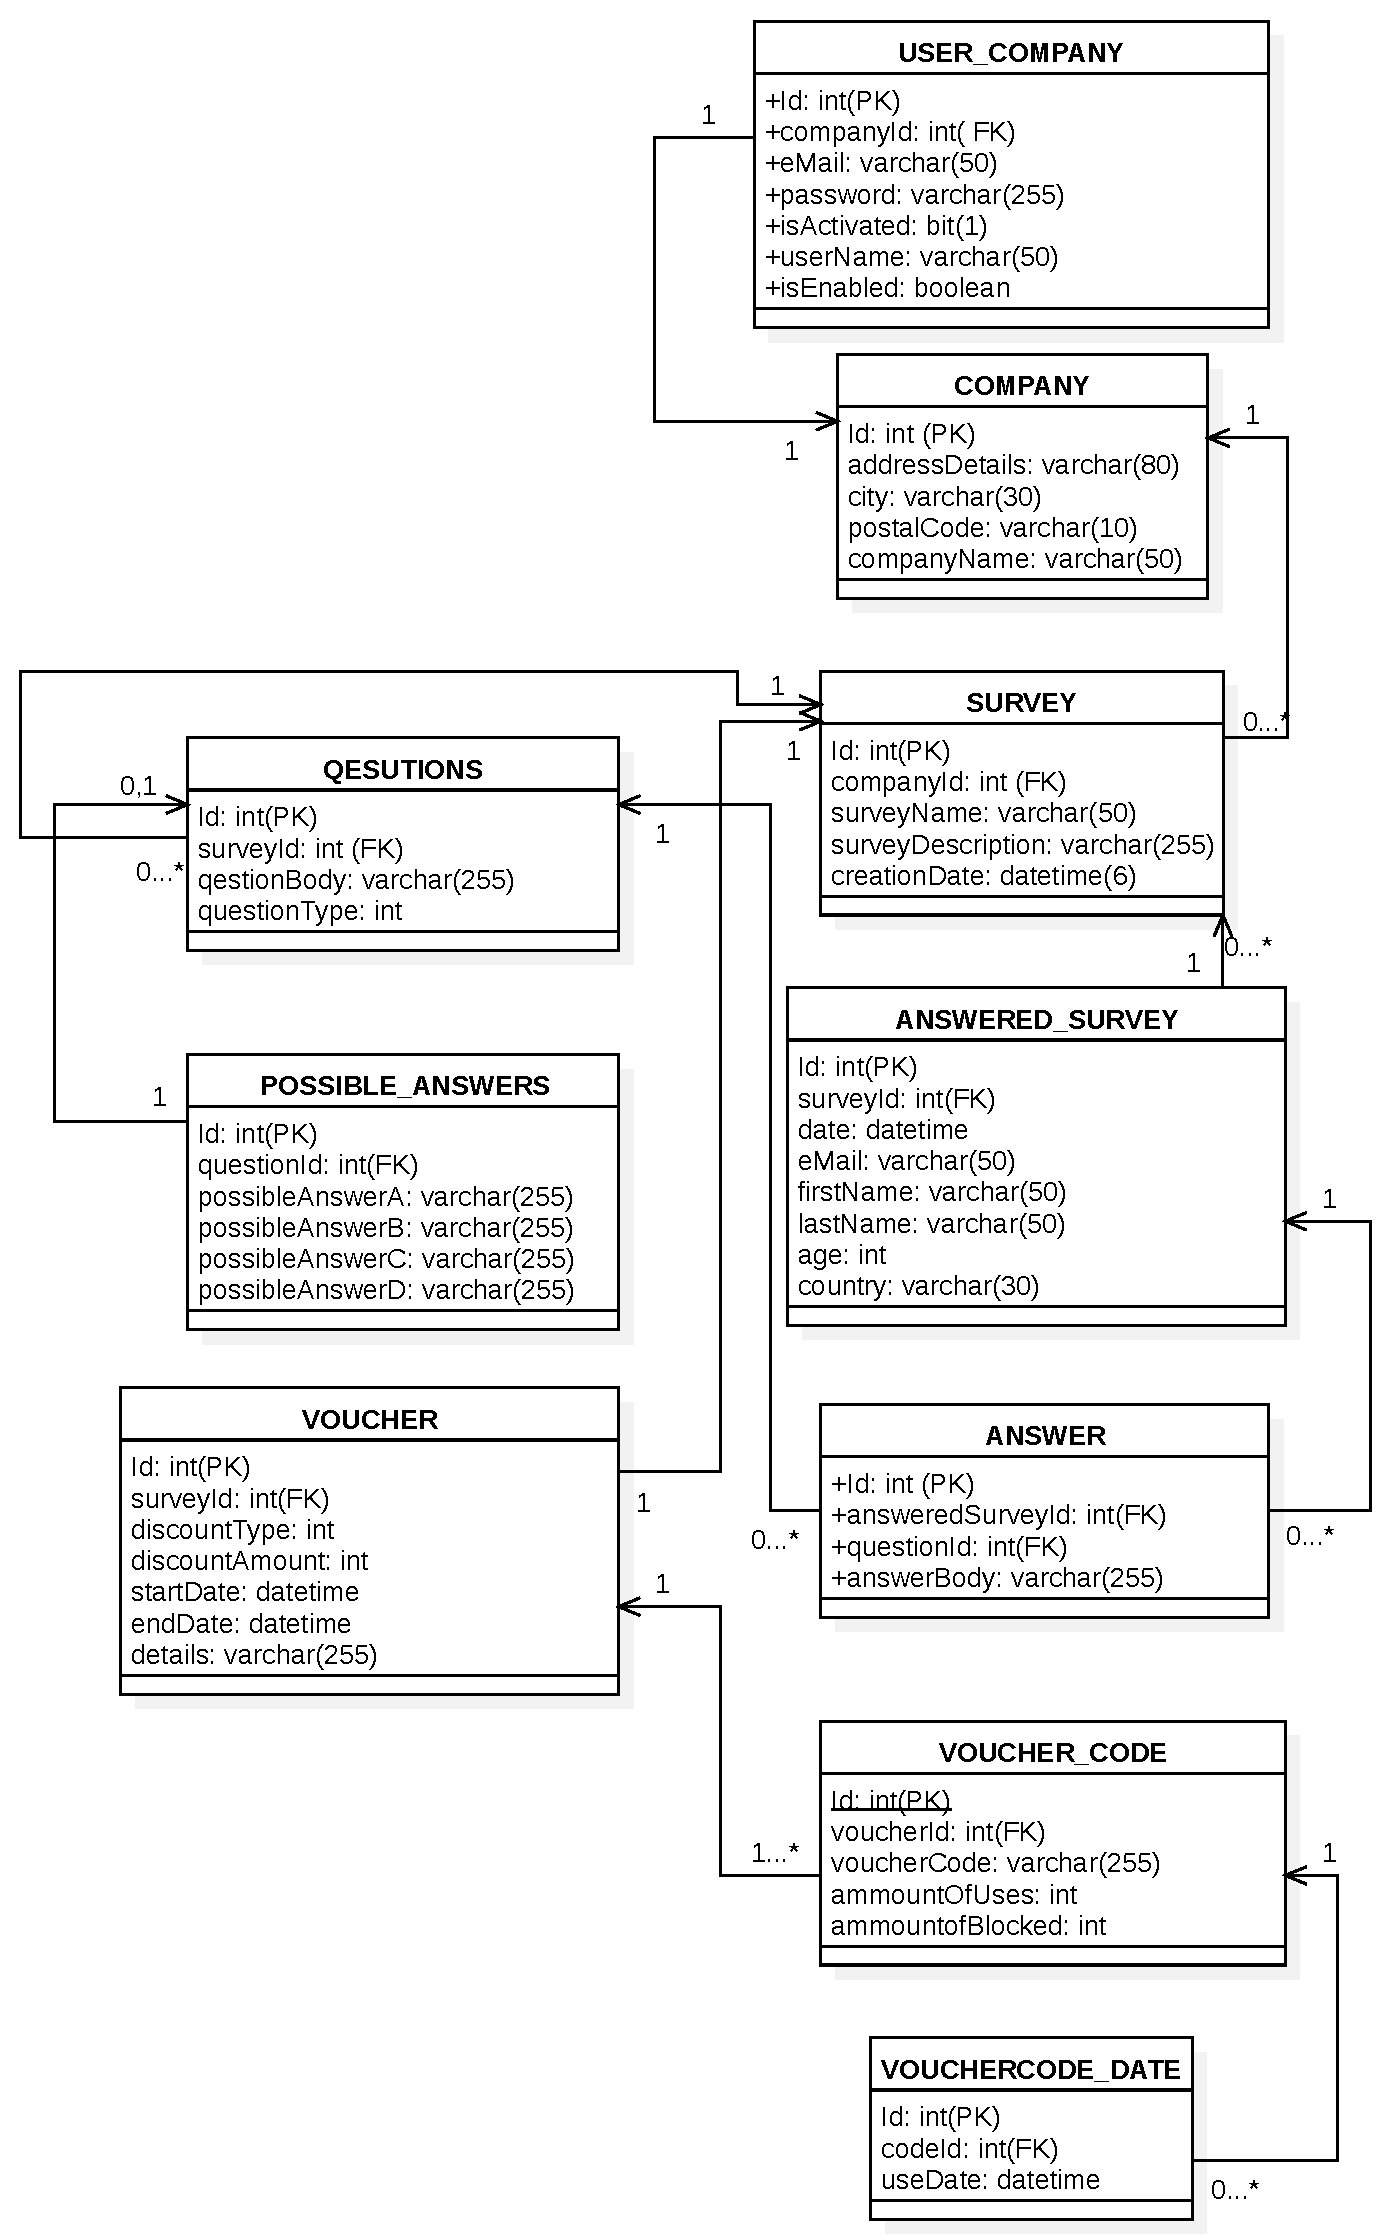
\includegraphics[scale=0.6]{db_diagram.pdf}
  \caption{Diagram klas przedstawiający baze danych systemu}
\end{figure}
W celu odpowiedniego zrozumienia struktury naszej aplikacji koniecznie jest zaznajomienie się kilkoma kluczowymi założeniami naszego systemu, którego miały bezpośredni wpływ na sposób w jaki zaprojektowaliśmy baze danych. Najważniejszym założeniem było przypisanie tylko i wyłącznie jednego typu kupony do jednej ankiety. Żadna ankieta może oferować tylko wyłacznie jeden typ kupony jako nagrodę za wypełnienie ankiety. Każdy voucher (który reprezentuje typ nagrody) może już miec przypisany więcej niż jeden kupon, każdy z nich może byc wielokrotnego użytku ( wtedy należy zaznaczyć jak wiele osób z niego może skorzystać) lub też jednorazowego użytku.
\linebreak
Równie ważnym założeniem było stworzenie tablicy \textbf{VoucherCode\_Date}, który odpowiada za ``blokowanie'' kupony na czas wypełnienia ankiet.
\subsection{Opis protokołów}
Ruch po naszej aplikacji ma miejsce przy użyciu protokołu \textbf{TLS}. Co ważne dostęp do każdej podusługi lub też podstrony naszego systemu wymaga połączenia zabezpieczonego, a użytkwonik chcący korzystać z naszej aplikacji przy użyciu protokołu \textbf{HTML} jest automatycznie przekierowywany na odpowiednią strone, która wykorzystuje już \textbf{TLS}. Podobno sytuacja ma miejsce z aplikacją mobilną, której połączenie z serwerem ma miejscu przy użyciu \textbf{TLS}.
\linebreak
Część aplikacji webowej dbająca o uwierzytelnianie	oraz autoryzacje (ang. authentication and authorization) przychodzących połączeń są filtry, które możemy uznać za protokół. Są one częścią \textbf{Servlet'ów}, która ma za zadanie jak sama nazwa wskazuje filtrować przychodzące zapytania, jak również w zależności od samego zapytania w odpowiedni sposób reagować. Informacje zawarte w zapytaniach oraz odpowiedziach serwera, które zostają dynamicznie przechowycone przez filtry są wykorzystywane między innymi do tego aby zidentyfikować autora zapytania (autoryzacja) i jeżeli będzie taka konieczność nadać mu odpowiednie uprawnienia (uwierzytelnienie). Jednym z zaimplementowanych przez nas zabezpieczeniem jest autoryzacja na poziomie metod serwisowych, jak również nadawanie ról użytkownikom w zależności od typu uprawnienień, które posiadają. Każdej osboie korzystającej z naszej aplikacji zostaje nadany unikatowy indetyfikator sesji, którym zostaje powiązany on i uprawnienia, które posiada. Właśnie te informacje wykorzystuje \textbf{The Security Filter Chain}, który jest częścią jednego z używanych przez nas narzędzi. Kiedy użytkownik legitymuje się swoim identyfikatorem sesji \textbf{The Security Filter Chain} (od tego momentu nazywany filtrem w celu zwiększenia czytelności tekstu) sprwadza w bazie danych czy istnieje już powiązane z tym identyfikatorem połączenie, w przypadku gdy zostanie to potwierdzone filter sprawdza jakie uprawnienia posiada to połączenie, skutkuje to powiązaniem uwierzytelnieniu zapytania przychodzącego do serwera, co następnie umożliwia wykorzystanie autoryzacji na poziomie metod, która sprawdza czy nasze uprawnienia są wystarczające.
\linebreak
Każdy użytkownik aplikacji webowej posiada odgórnie pewne uprawnienia, a w przypadku zalogowania się następuje dodatkowe uwierzytelnienie, gdzie jego identyfikator sesji wiązany z kontem do którego jest aktualnie zalogowany. To właśnie dzięki temu filter bezpieczeństwa potrafi jednoznacznie potwierdzić czy przychodzące zapytanie legitymujące się jedynie identyfikatorem sesji ma wystarczające uprawnienia do danej podusługi.
\linebreak
Ze względu na taki a nie inny sposób uwierzytelniania oraz autoryzacji konieczne również było użycie dodatkowego zabezpieczenia w postaci losowych tokenów chroniących przed atakami \textbf{CSRF} (ang. Cross-site request forgery), które w trakcie generowania zostają powiązane z identyfikatorem sesji, na którego życzenie zostały wygenerowane. Każdy użytkownik naszego serwisu podczas zapytań typu \textbf{POST} (sytuacja taka ma najczęściej miejsce podczas zatwierdzaniu różnego typu danych do serwera) musi ``wylegitymować się'' wygenerowanym wcześniej dla niego \textbf{CSRF tokenem} jak również identyfikatorem sesji, dopiero wtedy filter bezpieczeństwa zatwierdza takie zapytanie i przekazuje je do warstwy kontrolerów.
\linebreak
Częścią naszego systemu jest serwis mailowy, przez który jesteśmy w stanie komunikować się z klientami. Korzysta on z protkołu \textbf{STMP}.
\section{Implementacja systemu}
\subsection{Użyte technologie}
Całość systemu została zaimplementowana w jęzku obiektowym \textbf{Java 8} przy użyciu narzędzi dostępnych w \textbf{Java EE} (ang. enterprise edition). Do automatyzacji budowania projektu w przypadku aplikajci webowej został wykorzystany \textbf{Maven}, natomiast jeśli chodzi o aplikacje webową był to \textbf{Gradle}. Framework w oparciu którego została napisana aplikacja mobilna jest \textbf{Retrofit}. Ułatwia on w znaczny sposób pracę z różnego typu HTML'owych API (ang. application programming interface), m.in REST API. Narzędzie w znaczny sposób ułatwiło nam mapowanie obiket na JSON'a oraz JSON'a na obiekty, jak również samo wysyłanie zapytań oraz odbieranie i interpretacja odpowiedzi serwera, pamietając o konieczności legitymacji się identyfikatorem sesji.
\linebreak
Jeśli chodzi o część systemu odpowiedzialną za aplikacje webową technologiami, które zostały wykorzystane są narzędzia z rodziny \textbf{Spring}. Program został zaprojektowany zgodnie z zasadami \textbf{GRASP},a podczas implementacji z zachowaniem tych zasadł pomógł nam \textbf{Spring Core}, ułatwiał on wykorzystanie wzorca \textbf{DI} (ang. Dependency Injection), co skutkowało zachowaniem niskiego sprzężenia oraz wyskokiej spójności klas. Znaczna większość obiektów, które były wstrzykiwane poprzez \textbf{DI} były przedstawicielami wzorca projektowego \textbf{Singleton}, co skutowało zmniejszeniem zapotrzebania na zasoby komputera naszego serwera. Singletonami są wszystkie klasy serwisowe, kontrolery oraz klasy konfiguracyjne. Poza klasami konfiguracyjnymi wszystkie klasy wstrzykiwane przy użyciu \textbf{Spring Core} były implementacjami interfesjów, co pozwoliło \textbf{Springowi} w bardzo lekki i łatwy sposób przy użyciu refleksji budowanie \textbf{Proxy} tych obiektów w trakcie uruchomienia aplikacji i załadowania kontekstu,a nie jak miałoby by to miejsce w przypadki gdyby obiekty wstrzykiwane rozszerzały klase (lub też nie rozserzały żadnej kalsy abstrakcyjnej) modyfikując kod bitowy, który został wcześniej skompilowany. W różnych częsiach projektu mieliśmy doczynienia z programowaniem aspektowym, które również było możliwe, dzięki \textbf{Spring Core} oraz wcześniej stworzonym \textbf{Proxy} do wstrzykiwanych klas. Framework, z którym najwięcej pracowaliśmy to \textbf{Spring MVC}. Jest to narzędzie, które umożliwia z jasny sposób budować aplikacje webowe w opraciu o wzorzec projektowy \textbf{MVC}. Dzięki niemu w łatwy sposób mogliśmy zbudować most łączący widok z modelem, czyli kontrolery. \textbf{Spring MVC} rownież ułatwił nam walidacje dancyh otrzymanych przez użytkowników poprzez pare na adnotacjach dostępnych w pakietach \textbf{javax.validation.api}. Wraz z \textbf{Spring MVC} wykorzystywany był \textbf{Jackson}, czyli biblioteka odpowiedzialana za mapowanie instancje klas na obiekty JSON, oraz w drugą stronę.
\linebreak
W zabezpieczaniu naszego systemu pomogły nam rownież \textbf{Spring Security} oraz \textbf{Spring Session}. Drugie z nich dawało nam większą kontrole nad sesjami i jej atrybutami (tak jak \textbf{CSRF tokeny} oraz blokowane kupony, które rownież wiązane były z sesją) jak również umożliwiało nam to przechowywanie identyfiaktorów sesji w bazie danych. Jeśli chodzi o \textbf{Spring Security} miał on wpływ na implementacja autoryzacji oraz uwierzytelniania w naszym serwisie. To narzędzie sprawdzało podczas otrzymania zapytania przez serwer, czy dany użytkownik legitymujący się identyfikatorem sesji ma odpowiednie uprawnienia do przeglądania danej podstrony jak również wywoływania metod zarówna w kontrolerze oraz w klasach serwisowych. Umożliwił w łatwy sposób również implementacje różnego typu handler'ów dla przypadków, gdy użytkownikowi nie udało się prawdiłowo zalogować/wylogować lub gdy właśnie probował przejść do strony, do której nie ma dostępu. Narzędzie to również automatycznie hashuje hasła podane przez użytkowników (po wcześniejszym zadeklarowaniu wybranego przez nas algorytmu haszującego), co jest znaczące jeśli chodzi o przechowywanie wrażliwych dla użytkoników danych.
\linebreak
Kolejnym narzędziem jest \textbf{Thymeleaf}, który został wykorzystanu do front-end'owej częsci projektu, czyli silnik umożliwiający tworzenie szablonów HTML, który jest w łatwy sposób jest integrowany ze \textbf{Spring MVC}.  Dzięki możliwości korzystania m.in. z pętl, branch'ów oraz fragmentów kod HTML'owy stworzony przy użyciu Thymeleafa jest spójny oraz czytelny, gdyż miejscami przypomina kod jakiegoś standardowego języka programowania. Podczas prac nad modelem zostały wykorzystane również : \textbf{JavaScript},\textbf{jQuery},\textbf{CSS}.
\linebreak
Przydatnym narzędziem okazały się również \textbf{Spring WebFlow} oraz \textbf{Spring Mail}, które oferują wysokopoziomowe interfejsy dla wielostopniowych formularzy (ang. wizards) oraz wysyłce maili o zadanych wcześniej wyglądach (szablonach HTML). Pełna integracja z kodem Javowym w narzędziu odpowiedzialnym za formularze jest nie do opisania, ponieważ dzięki temu w formularzach jesteśmy wstanie zastosować branche, pracować na wprowadzonych przez użytkownika danych, jak również je przetwarzać na każdym etapie wykonywania formualrza.
\linebreak
Narzędziami przez nas użytymi były rownież frameworki ORM (ang. Object-Relational Mapping), a chodzi tu o \textbf{Hibernate}. Poprzez właśnie to narzędzie następowała komunikacja z naszą bazą danych \textbf{MySQL}, czyli wprowadzanie,edycja oraz usuwanie danych. \textbf{Hibernate} odpowiedzialny był za mapowanie krotek bazodanowych na instacje klas Modelu oraz instacji klas modelu na zapytania SQL'owe. Wykorzystany został rownież do wygenerowania gotowej bazy danych, na której później pracowaliśmy.
\subsection{Obliczanie statystyk}
\begin{lstlisting}[language=Java,tabsize=2,frame=single,breaklines=true]  
@Cacheable("surveyStat")
@Override
public SurveyStatisticsDto getSurveysStatistics(int surveyId) {
	Collection<AnsweredSurvey> answeredSurveys = getAllAnsweredSurveysWithDetails(surveyId);
	Survey survey = companySurveyService.getSurveyByIdWithQuestion(surveyId);
	SurveyStatisticsDto surveyStatisticsDto = new SurveyStatisticsDto();
	surveyStatisticsDto.setAmmount(answeredSurveys.size());
	surveyStatisticsDto.setSurveyName(survey.getSurveyName());

	//average age
	double averageAge = answeredSurveys.stream().mapToInt(a -> a.getUser().getAge()).average().orElse(0.0);
	surveyStatisticsDto.setAge(averageAge);

	//average country
	List<String> countries = answeredSurveys.stream().map(a -> a.getUser().getCountry()).collect(Collectors.groupingBy(Function.identity(), Collectors.counting())).entrySet().stream().sorted(Comparator.comparingLong(Map.Entry::getValue)).limit(3).map(Map.Entry::getKey).collect(Collectors.toList());
	while (countries.size() != 3)
		countries.add("N/A");
	surveyStatisticsDto.setCountry(countries.toArray(new String[3]));
	
	if (answeredSurveys.size() == 0)
		return surveyStatisticsDto;

	//initialaizing iterators
	Iterator<AnsweredSurvey> answeredSurveyIterator = answeredSurveys.iterator();
	Iterator<Question> qIterator = survey.getQuestions().iterator();
	Iterator<Answer>[] aIteratorArray = new Iterator[answeredSurveys.size()];
	IntStream.range(0, aIteratorArray.length).forEach(i -> aIteratorArray[i] = answeredSurveyIterator.next().getAnswersList().iterator());

	int answersSize = answeredSurveys.size();
	List<QuestionStatisticsDto> questionStatisticsDtoList = surveyStatisticsDto.getQuestionWithAnswersList();
	while (qIterator.hasNext()) {
		Question q = qIterator.next();
		QuestionType qType = q.getQuestionType();
		QuestionStatisticsDto questionStatisticsDto = new QuestionStatisticsDto();
		questionStatisticsDto.setQuestionBody(q.getQuestionBody());
		questionStatisticsDto.setQuestionType(qType);

		switch (qType) {
			case OPEN:
				Arrays.stream(aIteratorArray).forEach(Iterator::next);
				questionStatisticsDto.setAnswers(null);
				break;
			case RANGED:
				double average = 0;
				for (Iterator<Answer> anAIteratorArray : aIteratorArray) {
					String temp = anAIteratorArray.next().getAnswer();
					average += Double.parseDouble(temp);
				}
				questionStatisticsDto.getAnswers()[0].setAnswersStat(Double.toString(average / answersSize));
				break;
			default:
				double[] apperances = new double[4];
				for (Iterator<Answer> anAIteratorArray : aIteratorArray) {
					Answer a = anAIteratorArray.next();
					String[] splited = a.getAnswer().split(",");
					for (String s : splited) {
						switch (s) {
							case "A":
								apperances[0]++;
								break;
							case "B":
								apperances[1]++;
								break;
							case "C":
								apperances[2]++;
								break;
							case "D":
								apperances[3]++;
		           		}
					}
				}
				IntStream.range(0, apperances.length).forEach(a -> questionStatisticsDto.getAnswers()[a].setAnswersStat(Double.toString(100 * apperances[a] / answersSize)));
				questionStatisticsDto.setPossibleAnswers(q.getPossibleAnswers());
				break;
		}
            
		questionStatisticsDtoList.add(questionStatisticsDto);
	}
	return surveyStatisticsDto;
}
\end{lstlisting}
Na powyższym listingu warto zauwazyć, że metoda jest cache'owana tj. zapmietywane jest przez serwer wartość, która zostanie zwrócona dla danego argumentu. Przy dużej liczbie rozwiązanych ankiet obliczanie statystyk, może być stosunkow czasochłonne, a sam cache zapewnia nam, że nie statystyki dla tych samych danych nie będa liczone kilkukrotnie.
\paragraph{}
Pierwszym etapem jest pobranie z bazy danych listy wypełnionych ankiet, a następnie policzenie średniego wieku przy użyciu \textbf{Stream API}, \textbf{Lamba Expressions} oraz klasy generycznej \textbf{Optional<T>}. Przy użyiu tych samych ``narzędzi'' dostępnych w Javie zostaje obliczona posortowana lista krajów, względem częstości wypełniania danej ankiety w tym kraju. Lista ta jest ograniczona do $3$ najlepszych wyników, a w przypadku gdy zawiera ona mniej niż $3$ kraje zostaje wypełniona wyrażeniem ``N/A''. W przypadku gdy ankieta nie została rozwiązana zwracany jest pusty obiad, w innej sytuacji w pętli iterujemy po pytaniach w kolejnych odpowiedziach, tzn. na początku dla każdej odpowiedzi na pytanie numer $1$ liczymy statystyki, następnie robimy to dla każdej istniejącej odpowiedzi na pytanie numer $2$ itd. Jeżeli pytanie jest pytaniem typu ``ranged'' (tj. w skali od 0 do 10) liczona jest średnia arytmetyczna wyniku. Jeżeli jest to pytanie typu zamkniętego lub zamkniętego wieloktronego wyboru przy pomocy \textbf{Stream API}, \textbf{Lamba Expressions} oraz klasy generycznej \textbf{Optional<T>} liczona jest częstość występowania danej odpowiedzi (która należy do zbioru $\{A,B,C,D\}$). Następnie przy pomocy set'erów i get'erów klasy \textbf{SurveyStatisticsDto} obliczone wcześniej dane zostają ``wrzucone'' do obiektu wyjściowego, który jest ostatecznie zwracany przez metode.
\subsection{Restowanie hasła dla konta}
\begin{lstlisting}[language=Java,tabsize=2,frame=single,breaklines=true]
@RequestMapping(value = "forgot_password", method = RequestMethod.GET)
public String forgottenPassword(Model model) {
	model.addAttribute("form", new ForgotPasswordForm());
	return "auth/forgot_password.html";
}

@RequestMapping(value = "forgot_password", method = RequestMethod.POST)
public String forgottenPassword(@ModelAttribute(name = "form") @Validated ForgotPasswordForm forgotPasswordForm, BindingResult bindingResult) {
	if (bindingResult.hasErrors())
		return "auth/forgot_password.html";

	UserCompany userCompany = userCompanyService.getUserByUserName(forgotPasswordForm.getUserName());
	if (userCompany == null) {
		bindingResult.rejectValue("userName", "email.dont.exist", messageSource.getMessage("message.wrong.email", null, LocaleContextHolder.getLocale()));
		return "auth/forgot_password.html";
	} else if (!userCompany.isEnabled()) {
		bindingResult.rejectValue("userName", "account.not.activated", messageSource.getMessage("messages.account.not.activated", null, LocaleContextHolder.getLocale()));
		return "auth/forgot_password.html";
	} else {
		PasswordResetToken passwordResetToken = tokenService.generateNewPasswordResetToken(userCompany);
		mailService.sendPasswordResetEmail(passwordResetToken.getToken(), userCompany.getUsername());
	}

	return "redirect:/?acc=5";
}
\end{lstlisting}
Metoda oznaczona adnotacją $@RequestMapping(value = "/reset_password", method = RequestMethod.GET)$ przygotowywuje pusty formularz który ma zawierać jedynie adres e-mail konta dla którego użytkownik chce zresetować hasło. W przypadku, gdy użytkownik poda adres e-mail, który faktycznie znajduje się w naszej bazie danych zostaje generowany jednorazowy token (co zostało przedstawione w listingu poniżej), który zostaje wysłany w mail'u na wcześniej wskazany adres e-mail.
\begin{lstlisting}[language=Java,tabsize=2,frame=single,breaklines=true]
@Override
public PasswordResetToken generateNewPasswordResetToken(UserCompany userCompany) {
	tokenDao.deleteUsersResetTokens(userCompany.getUsername());
	PasswordResetToken passwordResetToken = new PasswordResetToken();
	passwordResetToken.setUserCompany(userCompany);
	passwordResetToken.setToken(RandomString.make(TOKEN_LENGTH));
	tokenDao.addPasswordResetToken(passwordResetToken);
	return passwordResetToken;
}

@Override
public PasswordResetToken validatePasswordResetToken(String passwordResetToken) throws WrongTokenException {
	try {
		return tokenDao.getPasswordResetTokenByToken(passwordResetToken);
	} catch (NoResultException ex) {
		throw new WrongTokenException();
	}
}
\end{lstlisting}
Tylko i wyłącznie jeden token odpowiadający za resetowanie hasła może być pisany do konta, tak więc przed dodaniem nowego ``PasswordResetToken'' ewentualny obiekt, który mógł istnieć wcześniej jest kasowany.
\begin{lstlisting}[language=Java,tabsize=2,frame=single,breaklines=true]
@RequestMapping(value = "/reset_password", method = RequestMethod.GET)
public String resetPassword(@RequestParam("t") String token, Model model) {
	try {
		tokenService.validatePasswordResetToken(token);
		ResetPasswordForm form = new ResetPasswordForm();
		form.setResetPasswordToken(token);
		model.addAttribute("resetPasswordForm", form);
		model.addAttribute("tokenStatus", TokenStatus.OK);
	} catch (WrongTokenException ex) {
		model.addAttribute("tokenStatus", TokenStatus.WRONG);
	}
	return "token/reset_password.html";
}

@RequestMapping(value = "/reset_password", method = RequestMethod.POST)
public String resetPassword(@ModelAttribute @Validated ResetPasswordForm resetPasswordForm, BindingResult bindingResult, Model model) {
	if (bindingResult.hasErrors()) {
		try {
			tokenService.validatePasswordResetToken(resetPasswordForm.getResetPasswordToken());
			model.addAttribute("tokenStatus", TokenStatus.OK);
		} catch (WrongTokenException ex) {
			model.addAttribute("tokenStatus", TokenStatus.WRONG);
		}
		return "token/reset_password.html";
	}
	userCompanyService.changePassword(resetPasswordForm);
	return "token/reset_password_success.html";
}
\end{lstlisting}
Użytkownik klikający w link w mailu wysłanym przez nasz system przekazujemy w postaci parametru zapytani $GET$ wcześniej wygenerowany token. Po wcześniejszej walidacji tokenu użytkwonik jest przeniesiony do strony zawierający formularz, w którym podaje dwa razy to samo nowe hasło, którym od momentu potwierdzenia formularza będzie się posługiwał.
\subsection{Rejestracja}
Do implementacji mechanizmu rejestracji zostało wykorzystane narzędzie o nazwie \textbf{Spring WebFlow}, które jest wykorzystywane do wielostopniowego formularza (ang. wizard). W pliku XML-owym możemy odwoływac się do metod serwisowych, implementować na podstawie tego branch'e oraz decydowac na jakim etapie formularza jaka grupa walidacji będzie walidowana.
\begin{lstlisting}[language=XML,tabsize=2,frame=single,breaklines=true]
<?xml version="1.0" encoding="UTF-8"?>
<flow xmlns="http://www.springframework.org/schema/webflow"
      xmlns:xsi="http://www.w3.org/2001/XMLSchema-instance"
      xsi:schemaLocation="http://www.springframework.org/schema/webflow http://www.springframework.org/schema/webflow/spring-webflow-2.4.xsd">

    <var name="company" class="pwr.groupproject.vouchers.bean.form.NewUserCompanyForm"/>

    <view-state id="step1" view="/signup/signup1.html" model="company"
                validation-hints="'validationGroup1'" >
        <transition on="nextStep" to="step2">
            <evaluate expression="userCompanyServiceImpl.validateUserCompany(company,messageContext)" />
        </transition>
        <transition on="cancel" to="cancel" validate="false" bind="false" />
    </view-state>

    <view-state id="step2" view="/signup/signup2.html" model="company"
                validation-hints="'validationGroup2'">
        <transition on="nextStep" to="success">
            <evaluate expression="userCompanyServiceImpl.addUser(company)" />
        </transition>
        <transition on="cancel" to="cancel" validate="false" />
        <transition on="previousStep" to="step1" validate="false" />
    </view-state>

    <end-state id="success" view="externalRedirect:/?acc=1" />
    <end-state id="cancel" view="externalRedirect:/" />
</flow>
\end{lstlisting}
Dla pierwszego etapu rejestracji do modelu (który jest ten sam dla całego trwania procesu) dodawany jest pusty formularz, czyli obiekt w którym będziemy przechowywać wszystkie dane wprowadzone przez użytkownika. Następnie po zatwierdzeniu pierwszego etapu przez użytkownika , sprwadzamy czy wprowadzone dane są zgodne z wymogami przedstawionymi przez serwer (np. czy podany przez użytkownika adres e-mail nie znajduje się już w naszej bazie danych) poprzez $<evaluate expression="userCompanyServiceImpl.validateUserCompany(company,messageContext)" />$,  w której wywołujemy klase serwisową naszego systemu. W przypadku, gdy dane nie spełnią wymogów wyświetlamy odpowiednie komunikaty błędów, w których jasno informujemy klienta co należy zrobić, aby owe wymogi spełnić. W przypadku gdy dane zostaną zatwierdzone przez serwer przechodzimy do drugiego etapu formularza  $<view-state id="step2" ... </view-state>$. Tam użytkownik uzupełnia formularz kolejną serią danych (np. hasłem oraz jego powtórzeniem) po zatwierdzeniu których serwer poraz kolejny waliduje dane wejściowe, tym razem już cały formularz. W przypadku przejścia wszystkich wymogów walidacji zostaje wykonana instrukcja $<transition on="nextStep" to="success">...</transition>$, co skutkuje wywołanem funkcji serwisowej $addUser(obj: Company)$. Po pomyślnym dodaniu użytkownika do bazy danych proces trafia do linijki $25$ w powyższym listingu i zostaje przekierowany na strone startową, na której dzięki parametrowi ``acc'' wyświetli się odpowiedni komunikat informujący o konieczności aktywacji konta przed zalogowaniem się.
\end{document}
